\documentclass[a4paper,12pt]{article}
\usepackage[utf8]{inputenc}
\usepackage[T2A]{fontenc}
\usepackage[english,russian]{babel}
\title{Произвольная производная, потенциально повергающая.}
\author{просто проект}

\usepackage{natbib}
\usepackage{graphicx}

\usepackage{amsmath,amsfonts,amssymb,amsthm,mathtools}
\usepackage{icomma} 

\mathtoolsset{showonlyrefs=true}

\usepackage{euscript} 
\usepackage{mathrsfs} 
%\usepackage{graphicx}
\graphicspath{{./pictures/}}
\DeclareGraphicsExtensions{.pdf,.png,.jpg}

\DeclareMathOperator{\sgn}{\mathop{sgn}}


\begin{document}

\maketitle

ломать не строить, дифференцировать - не угадывать функцию 

$(x)'$

$1$

если бы мы поставили пять штрихов, то латех бы расстроился 

$(x)'$

$1$

  

$(x^{x})'$

$x^{x} \cdot ( \frac{1}{x}  \cdot x+ \ln x \cdot 1)$

  

$(x)'$

$1$

умение брать производные не убавит вам причин идти на производство 

$(x^{2})'$

$2 \cdot 1 \cdot x^{1}$

  

$(x)'$

$1$

если кафедра Выш Мата увидела бы это, то она бы расстроилась 

$(x+x^{2})'$

$1+2 \cdot 1 \cdot x^{1}$

хорошо, что мы берем производную, ведь интегрировать мы не умеем 

$(3)'$

$0$

на глаз проводим касательную 

$(3+x+x^{2})'$

$0+1+2 \cdot 1 \cdot x^{1}$

один штрих, а столько проблем... 

$(x)'$

$1$

на глаз проводим касательную 

$(2)'$

$0$

если кафедра Выш Мата увидела бы это, то она бы расстроилась 

$(2 \cdot x)'$

$0 \cdot x+2 \cdot 1$

  

$(x)'$

$1$

на глаз проводим касательную 

$( \th x)'$

$ \frac{1}{( \ch x)^{2}} $

один штрих, а столько проблем... 

$(1)'$

$0$

  

$(1+ \th x)'$

$0+ \frac{1}{( \ch x)^{2}} $

если бы мы поставили пять штрихов, то латех бы расстроился 

$((1+ \th x)^{2 \cdot x})'$

$(1+ \th x)^{2 \cdot x} \cdot ( \frac{0+ \frac{1}{( \ch x)^{2}} }{1+ \th x}  \cdot 2 \cdot x+ \ln (1+ \th x) \cdot (0 \cdot x+2 \cdot 1))$

Иисус научил меня превращать выражение в воду 

$( \frac{(1+ \th x)^{2 \cdot x}}{3+x+x^{2}} )'$

$ \frac{(1+ \th x)^{2 \cdot x} \cdot ( \frac{0+ \frac{1}{( \ch x)^{2}} }{1+ \th x}  \cdot 2 \cdot x+ \ln (1+ \th x) \cdot (0 \cdot x+2 \cdot 1)) \cdot (3+x+x^{2})-(1+ \th x)^{2 \cdot x} \cdot (0+1+2 \cdot 1 \cdot x^{1})}{(3+x+x^{2})^{2}} $

если кафедра Выш Мата увидела бы это, то она бы расстроилась 

$( \frac{(1+ \th x)^{2 \cdot x}}{3+x+x^{2}} +x^{x})'$

$ \frac{(1+ \th x)^{2 \cdot x} \cdot ( \frac{0+ \frac{1}{( \ch x)^{2}} }{1+ \th x}  \cdot 2 \cdot x+ \ln (1+ \th x) \cdot (0 \cdot x+2 \cdot 1)) \cdot (3+x+x^{2})-(1+ \th x)^{2 \cdot x} \cdot (0+1+2 \cdot 1 \cdot x^{1})}{(3+x+x^{2})^{2}} +x^{x} \cdot ( \frac{1}{x}  \cdot x+ \ln x \cdot 1)$

если бы мы поставили пять штрихов, то латех бы расстроился 

$(x)'$

$1$

да, я слышал про производные... не знал, что их надо производить 

$(1)'$

$0$

умение брать производные не убавит вам причин идти на производство 

$( \frac{1}{x} )'$

$ \frac{0 \cdot x-1 \cdot 1}{x^{2}} $

ломать не строить, дифференцировать - не угадывать функцию 

$( \sin ( \frac{1}{x} ))'$

$ \cos ( \frac{1}{x} ) \cdot  \frac{0 \cdot x-1 \cdot 1}{x^{2}} $

ломать не строить, дифференцировать - не угадывать функцию 

$(x)'$

$1$

если кафедра Выш Мата увидела бы это, то она бы расстроилась 

$(x \cdot  \sin ( \frac{1}{x} ))'$

$1 \cdot  \sin ( \frac{1}{x} )+x \cdot  \cos ( \frac{1}{x} ) \cdot  \frac{0 \cdot x-1 \cdot 1}{x^{2}} $

ломать не строить, дифференцировать - не угадывать функцию 

$(x \cdot  \sin ( \frac{1}{x} )+ \frac{(1+ \th x)^{2 \cdot x}}{3+x+x^{2}} +x^{x})'$

$1 \cdot  \sin ( \frac{1}{x} )+x \cdot  \cos ( \frac{1}{x} ) \cdot  \frac{0 \cdot x-1 \cdot 1}{x^{2}} + \frac{(1+ \th x)^{2 \cdot x} \cdot ( \frac{0+ \frac{1}{( \ch x)^{2}} }{1+ \th x}  \cdot 2 \cdot x+ \ln (1+ \th x) \cdot (0 \cdot x+2 \cdot 1)) \cdot (3+x+x^{2})-(1+ \th x)^{2 \cdot x} \cdot (0+1+2 \cdot 1 \cdot x^{1})}{(3+x+x^{2})^{2}} +x^{x} \cdot ( \frac{1}{x}  \cdot x+ \ln x \cdot 1)$

Функция без упрощения:

$1 \cdot  \sin ( \frac{1}{x} )+x \cdot  \cos ( \frac{1}{x} ) \cdot  \frac{0 \cdot x-1 \cdot 1}{x^{2}} + \frac{(1+ \th x)^{2 \cdot x} \cdot ( \frac{0+ \frac{1}{( \ch x)^{2}} }{1+ \th x}  \cdot 2 \cdot x+ \ln (1+ \th x) \cdot (0 \cdot x+2 \cdot 1)) \cdot (3+x+x^{2})-(1+ \th x)^{2 \cdot x} \cdot (0+1+2 \cdot 1 \cdot x^{1})}{(3+x+x^{2})^{2}} +x^{x} \cdot ( \frac{1}{x}  \cdot x+ \ln x \cdot 1)$

Иисус научил меня превращать воду в выражение 

$ \frac{1}{x}  \cdot x+ \ln x \cdot 1$

$ \frac{1}{x}  \cdot x+ \ln x$

здесь должна быть ваша реклама 

$2 \cdot 1 \cdot x^{1}$

$2 \cdot x^{1}$

только гении поймут эту простату 

$0 \cdot x+2 \cdot 1$

$0 \cdot x+2$

спасибо деду за дифуры, пойду ка разгружать я фуры (не мое) 

$0 \cdot x-1 \cdot 1$

$0 \cdot x-1$

здесь должна была быть смешная фраза 

$1 \cdot  \sin ( \frac{1}{x} )+x \cdot  \cos ( \frac{1}{x} ) \cdot  \frac{0 \cdot x-1}{x^{2}} $

$ \sin ( \frac{1}{x} )+x \cdot  \cos ( \frac{1}{x} ) \cdot  \frac{0 \cdot x-1}{x^{2}} $

спасибо деду за дифуры, пойду ка разгружать я фуры (не мое) 

$0 \cdot x$

здесь должна была быть смешная фраза 

$0 \cdot x$

здесь должна была быть смешная фраза 

$(1+ \th x)^{2 \cdot x} \cdot (0+1+2 \cdot x^{1})$

$(1+ \th x)^{2 \cdot x} \cdot (1+2 \cdot x^{1})$

Иисус научил меня превращать воду в выражение 

$ \ln (1+ \th x) \cdot (0+2)$

$ \ln (1+ \th x) \cdot 2$

здесь должна была быть смешная фраза 

$ \frac{0+ \frac{1}{( \ch x)^{2}} }{1+ \th x} $

$ \frac{ \frac{1}{( \ch x)^{2}} }{1+ \th x} $

вольфрам сделал бы это быстрее, но мы хотя бы смогли 

$0-1$

$-1$

ИТОГ:

$ \sin ( \frac{1}{x} )+x \cdot  \cos ( \frac{1}{x} ) \cdot  \frac{-1}{x^{2}} + \frac{(1+ \th x)^{2 \cdot x} \cdot ( \frac{ \frac{1}{( \ch x)^{2}} }{1+ \th x}  \cdot 2 \cdot x+ \ln (1+ \th x) \cdot 2) \cdot (3+x+x^{2})-(1+ \th x)^{2 \cdot x} \cdot (1+2 \cdot x^{1})}{(3+x+x^{2})^{2}} +x^{x} \cdot ( \frac{1}{x}  \cdot x+ \ln x)$



Выводим невероятный ряд тейлора с остаточным членом в форме ))))))

$f(x) = 2.46 + \frac{1.93}{1!} \cdot (x - 1) + \frac{1.84}{2!} \cdot (x - 1)^{2} + \frac{6.25}{3!} \cdot (x - 1)^{3} + \frac{-4.92}{4!} \cdot (x - 1)^{4} + \frac{80.7}{5!} \cdot (x - 1)^{5} + o((x - 1)^{6})$

Однако, все эти преобразования и мороки - сущая ерунда и пустая трата времени. наиболее надежный метод вычислить производную - чиркнуть на глаз касательную.

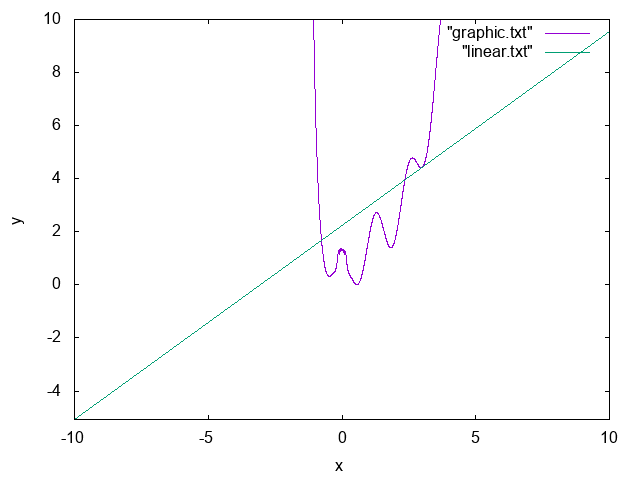
\includegraphics{graphic.png}\section{Список Литературы}

0. Репозиторий https://github.com/Krym4s

1. Деятели русской науки XIX - XX веков. Вып. 2 / РАН, Ин-т ист. естеств. и техники, Ин-т рос. истории; Отв. ред. И.П. Медведев. - СПб.: Дмитрий Буланин, 2001. - 414 с.

2. Сапрыкин Д. Л. Образовательный потенциал Российской Империи. М.:ИИЕТ, 2010

3. Организация науки в России в первой половине XIX века / Г.Е. Павлова; АН СССР, Ин-т истории естествознания и техники; Отв. ред. С.Р. Микулинский. - М. : Наука, 1990. - 239 с.

4. Деятели русской науки XIX - XX веков. Вып. 1 / РАН, Ин-т ист. естеств. и техники, Ин-т рос. истории; Отв. ред. И.П. Медведев. - СПб.: Дмитрий Буланин, 2001.

5. Образование и наука в первой половине XIX в. https://www.yaklass.ru/materiali?mode=lsnthemesubid=31themeid=165

6. 19 век в истории информатики https://intellect.icu/vek-v-istorii-informatiki-  6000

\end{document}